\documentclass[a4paper]{book}

\usepackage{geometry}
% make full use of A4 papers
\geometry{margin=1.5cm, vmargin={0pt,1cm}}
\setlength{\topmargin}{-1cm}
\setlength{\paperheight}{29.7cm}
\setlength{\textheight}{25.1cm}

% auto adjust the marginals
\usepackage{marginfix}

\usepackage{amsfonts}
\usepackage{amsmath}
\usepackage{amssymb}
\usepackage{amsthm}
%\usepackage{CJKutf8}   % for Chinese characters
\usepackage{ctex}
\usepackage{enumerate}
\usepackage{graphicx}  % for figures
\usepackage{layout}
\usepackage{multicol}  % multiple columns to reduce number of pages
\usepackage{mathrsfs}  
\usepackage{fancyhdr}
\usepackage{subfigure}
\usepackage{tcolorbox}
\usepackage{tikz-cd}
\usepackage{listings}
\usepackage{xcolor} %代码高亮
\usepackage{braket}
\usepackage{algorithm} 
\usepackage{algorithmicx}  
\usepackage{algpseudocode}  
\usepackage{amsmath}  

\floatname{algorithm}{算法}  
\renewcommand{\algorithmicrequire}{\textbf{输入:}}  
\renewcommand{\algorithmicensure}{\textbf{输出:}}  
\renewcommand{\algorithmicrequire}{\textbf{Input : }}
\renewcommand{\algorithmicrequire}{\textbf{Precondition : }}
\renewcommand{\algorithmicensure}{\textbf{Output : }}
\renewcommand{\algorithmicensure}{\textbf{Postcondition : }}
%------------------
% common commands %
%------------------
% differentiation
\newcommand{\gen}[1]{\left\langle #1 \right\rangle}
\newcommand{\dif}{\mathrm{d}}
\newcommand{\difPx}[1]{\frac{\partial #1}{\partial x}}
\newcommand{\difPy}[1]{\frac{\partial #1}{\partial y}}
\newcommand{\Dim}{\mathrm{D}}
\newcommand{\avg}[1]{\left\langle #1 \right\rangle}
\newcommand{\sgn}{\mathrm{sgn}}
\newcommand{\Span}{\mathrm{span}}
\newcommand{\dom}{\mathrm{dom}}
\newcommand{\Arity}{\mathrm{arity}}
\newcommand{\Int}{\mathrm{Int}}
\newcommand{\Ext}{\mathrm{Ext}}
\newcommand{\Cl}{\mathrm{Cl}}
\newcommand{\Fr}{\mathrm{Fr}}
% group is generated by
\newcommand{\grb}[1]{\left\langle #1 \right\rangle}
% rank
\newcommand{\rank}{\mathrm{rank}}
\newcommand{\Iden}{\mathrm{Id}}

% this environment is for solutions of examples and exercises
\newenvironment{solution}%
{\noindent\textbf{Solution.}}%
{\qedhere}
% the following command is for disabling environments
%  so that their contents do not show up in the pdf.
\makeatletter
\newcommand{\voidenvironment}[1]{%
\expandafter\providecommand\csname env@#1@save@env\endcsname{}%
\expandafter\providecommand\csname env@#1@process\endcsname{}%
\@ifundefined{#1}{}{\RenewEnviron{#1}{}}%
}
\makeatother

%---------------------------------------------
% commands specifically for complex analysis %
%---------------------------------------------
% complex conjugate
\newcommand{\ccg}[1]{\overline{#1}}
% the imaginary unit
\newcommand{\ii}{\mathbf{i}}
%\newcommand{\ii}{\boldsymbol{i}}
% the real part
\newcommand{\Rez}{\mathrm{Re}\,}
% the imaginary part
\newcommand{\Imz}{\mathrm{Im}\,}
% punctured complex plane
\newcommand{\pcp}{\mathbb{C}^{\bullet}}
% the principle branch of the logarithm
\newcommand{\Log}{\mathrm{Log}}
% the principle value of a nonzero complex number
\newcommand{\Arg}{\mathrm{Arg}}
\newcommand{\Null}{\mathrm{null}}
\newcommand{\Range}{\mathrm{range}}
\newcommand{\Ker}{\mathrm{ker}}
\newcommand{\Iso}{\mathrm{Iso}}
\newcommand{\Aut}{\mathrm{Aut}}
\newcommand{\ord}{\mathrm{ord}}
\newcommand{\Res}{\mathrm{Res}}
%\newcommand{\GL2R}{\mathrm{GL}(2,\mathbb{R})}
\newcommand{\GL}{\mathrm{GL}}
\newcommand{\SL}{\mathrm{SL}}
\newcommand{\Dist}[2]{\left|{#1}-{#2}\right|}

\newcommand\tbbint{{-\mkern -16mu\int}}
\newcommand\tbint{{\mathchar '26\mkern -14mu\int}}
\newcommand\dbbint{{-\mkern -19mu\int}}
\newcommand\dbint{{\mathchar '26\mkern -18mu\int}}
\newcommand\bint{
{\mathchoice{\dbint}{\tbint}{\tbint}{\tbint}}
}
\newcommand\bbint{
{\mathchoice{\dbbint}{\tbbint}{\tbbint}{\tbbint}}
}





%----------------------------------------
% theorem and theorem-like environments %
%----------------------------------------
\numberwithin{equation}{chapter}
\theoremstyle{definition}

\newtheorem{thm}{Theorem}[chapter]
\newtheorem{axm}[thm]{Axiom}
\newtheorem{alg}[thm]{Algorithm}
\newtheorem{asm}[thm]{Assumption}
\newtheorem{defn}[thm]{Definition}
\newtheorem{prop}[thm]{Proposition}
\newtheorem{rul}[thm]{Rule}
\newtheorem{coro}[thm]{Corollary}
\newtheorem{lem}[thm]{Lemma}
\newtheorem{exm}{Example}[chapter]
\newtheorem{rem}{Remark}[chapter]
\newtheorem{exc}[exm]{Exercise}
\newtheorem{frm}[thm]{Formula}
\newtheorem{ntn}{Notation}

% for complying with the convention in the textbook
\newtheorem{rmk}[thm]{Remark}


%\lstset{
%	backgroundcolor=\color{red!50!green!50!blue!50},%代码块背景色为浅灰色
%	rulesepcolor= \color{gray}, %代码块边框颜色
%	breaklines=true,  %代码过长则换行
%	numbers=left, %行号在左侧显示
%	numberstyle= \small,%行号字体
%	keywordstyle= \color{blue},%关键字颜色
%	commentstyle=\color{gray}, %注释颜色
%	frame=shadowbox%用方框框住代码块
%}
\lstset{
columns=fixed,       
numbers=left,                                        % 在左侧显示行号
numberstyle=\tiny\color{gray},                       % 设定行号格式
frame=none,                                          % 不显示背景边框
backgroundcolor=\color[RGB]{245,245,244},            % 设定背景颜色
keywordstyle=\color[RGB]{40,40,255},                 % 设定关键字颜色
numberstyle=\footnotesize\color{darkgray},           
commentstyle=\it\color[RGB]{0,96,96},                % 设置代码注释的格式
stringstyle=\rmfamily\slshape\color[RGB]{128,0,0},   % 设置字符串格式
showstringspaces=false,                              % 不显示字符串中的空格
language=c++,                                        % 设置语言
}

%----------------------
% the end of preamble %
%----------------------

\begin{document}
\pagestyle{empty}
\pagenumbering{roman}

%\tableofcontents
%\clearpage

%\pagestyle{fancy}
%\fancyhead{}
%\lhead{Qinghai Zhang}
%\chead{Notes on Algebraic Topology}
%\rhead{Fall 2018}


\setcounter{chapter}{0}
\pagenumbering{arabic}
% \setcounter{page}{0}

% --------------------------------------------------------
% uncomment the following to remove these environments 
%  to generate handouts for students.
% --------------------------------------------------------
% \begingroup
% \voidenvironment{rem}%
% \voidenvironment{proof}%
% \voidenvironment{solution}%


% each chapter is factored into a separate file.

\title{Boolean3D Document}

\chapter{类成员简介}
\section{Yinset}
\subsection{成员数据}
\textbf{vector<GluingClosedSurface> vecGCS}

这里存放了构成殷集边界的有向黏合紧曲面

\textbf{vector<HasseNode> Hasse}

存放了有向黏合紧曲面之间的包含关系
\subsection{成员函数}
\textbf{Yinset meet(const Yinset\&) const}

实现了两个殷集的求交

\textbf{Yinset join(const Yinset\&) const}

实现了两个殷集的求并

\textbf{Yinset complement() const}

实现了殷集求补集

\textbf{buildHasse()}

计算黏合紧曲面的包含关系,输出Hasse图


\section{GluingClosedSurface}
表示一个黏合紧曲面

\subsection{成员数据}
\textbf{vector<Triangle> vecTriangle}

存放了黏合紧曲面的三角剖分

\textbf{bool orientation}

存放了黏合紧曲面的方向

\section{SurfacePatch}
表示切割后的曲面片

\subsection{成员数据}
\textbf{vector<Triangle> vecTriangle}

存放了曲面片的三角剖分

\textbf{vector<pair<Segment> boundary}

存放了曲面片的边界

\subsection{成员函数}
\textbf{reverse()}

将曲面片反向,也就是将所有三角形的顶点顺序取反


\section{PrePaste}
实现了将曲面沿闭合交线切割成曲面片的过程


\subsection{成员数据}
\textbf{vector<GluingClosedSurface> vecGCS}

存放了不需要进行切割的黏合紧曲面

\textbf{vector<SurfacePatch> vecSP}

存放了切割以后得到的曲面片

\subsection{成员函数}
\textbf{operator()(const vector<Triangle>\&)}

将一个殷集中所有三角形放在一起作为输入,将这些三角形黏合起来,直到遇到边界,这个过程等效于将黏合紧曲面沿交线进行切割。


\section{Paste}
实现了将曲面片沿边界黏合成黏合紧曲面的过程



\subsection{成员函数}
\textbf{vector<GluingClosedSurface> operator()(const vector<SurfacePatch>\&)}

将输入的曲面片沿边界黏合成黏合紧曲面并输出

\section{Locate}

\subsection{成员函数}
\textbf{bool operator()(const Point\&, const GluingClosedSurface\&)}

判断一个点是否在一个黏合紧曲面的有界补集内部

\section{TriangleIntersect}

\subsection{成员数据}
vector<pair<vector<Segment>,
vector<vector<Triangle>::iterator>>> :
resultA, reasultB

存放了两个殷集的所有三角形之间相交的信息和重合的信息

\subsection{成员函数}
\textbf{operator()(const Triangle\&, const
Triangle\&)}

实现两个三角形的求交

\textbf{vector<Triangle> collapse()}
将所有三角形根据相交信息进行三角剖分

\section{Triangulate}

\subsection{成员函数}

\textbf{bool operator()(const Triangle\&, const vector<Segment>\&)}
将输入的三角形根据交线进行三角剖分


\section{Triangle}
实现了三角剖分所需的三角形


\subsection{成员数据}
\textbf{vector<Point> vecPoint}

存放了三角形三个顶点,顶点顺序与定向有关

% \textbf{vector<Edge> Edges}
% 存放了三角形的三条边
\textbf{pairt<int,int> InFace}
记录在哪一个曲面中

\subsection{成员函数}
\textbf{Triangle<2> project(int n)}

将三维空间三角形投影到某个坐标平面

\textbf{intersect(const Line\&)}

实现空间中三角形与一条直线求交

\textbf{intersectCoplane(const Line<2>\&)}
实现平面中三角形和直线求交

\textbf{Triangle reverse()}
将三角形顶点顺序反向


\section{Plane}
表示三角形所在平面


\subsection{成员数据}
\textbf{Real para[Dim+1]}

存放了平面方程的四个参数



\subsection{成员函数}
\textbf{ Real angle(const Plane\&)}

求两个平面的夹角

\textbf{Line intersect(const Plane\&}

实现两个平面求交,输出交的直线


\section{Line}
表示一条直线


\subsection{成员数据}
\textbf{Point fixPoint}

存放了直线上一点坐标

\textbf{Vec dirct}

存放了直线的方向向量


\subsection{成员函数}
\textbf{ Line<2> project(int n)}

将空间中直线投影到某个坐标平面


\section{Edge}
表示一条线段


\subsection{成员数据}
\textbf{Point endPoint[2]}

表示线段的两个端点



\subsection{成员函数}
\textbf{Edge<2> project(int n) }

将空间中线段投影到某个坐标平面


\section{Segment}
表示一条交线


\subsection{成员数据}
\textbf{Point endPoint[2]}

表示交线的两个端点

\textbf{vector<Triangle>}

存放了交线对应的两个三角形



\section{Point}
表示空间中一个点


\subsection{成员数据}
\textbf{Real coord[Dim]}

表示点的坐标


\section{Vec}
表示一个向量


\subsection{成员数据}
\textbf{Real p[Dim]}

表示向量的各个分量



\subsection{成员函数}
\textbf{Real dot(const Vec\&) }

实现向量点乘

\textbf{Real cross(const Vec\&) }

实现向量叉乘	
\begin{figure}
	\caption{UML类图}
	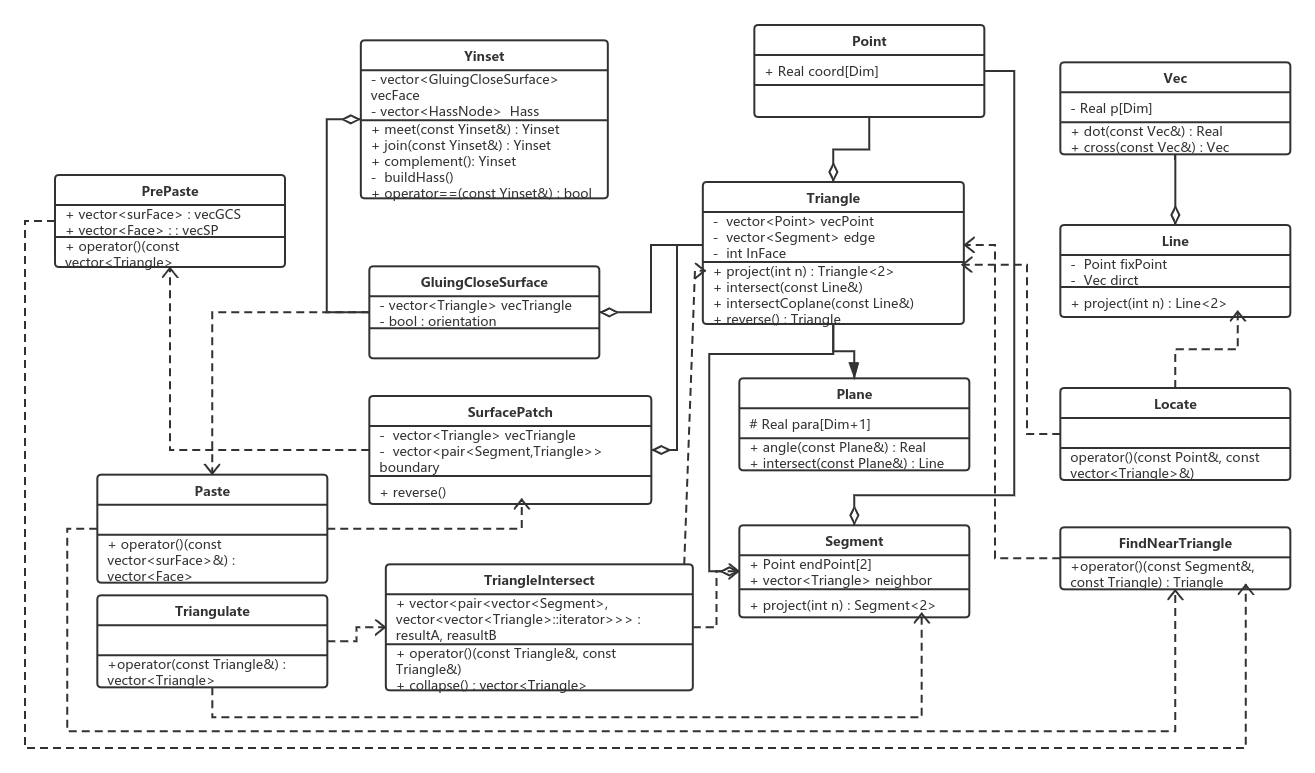
\includegraphics[width = 18cm]{fig/Boolean3D.png}
\end{figure}


\chapter{算法伪代码}

\section{算法证明}
\subsection{算法4: 寻找恰当的粘合三角形}
在确定恰当粘合三角形中,为了满足DEFINITION 2.11中的好配对.选取两个相邻的广义扇形
配对,在程序中即为两个相邻三角形.

这里定义相邻,两个三角形a,b公共一条边e且a,b在e上的方向相反.
a沿着边e,以a的法向量方向反方向旋转,与a共面的满足之上条件的所有三角形中b是第一个,
则称a,b相邻,易见b到a的旋转也满足条件,所以以相邻配对是唯一的.
又结合Yinset边界是闭曲面沿1维CW复形粘合结果,因此相邻配对是存在的.

2-7行得到两个共边三角形的法向量$normtri,normneightri$.不妨设为$A,B$,
\begin{align}
	&A * B = \lVert A \rVert \cdot \lVert B \rVert \cdot \cos(\alpha) \\
	&A \times B = \lVert A \rVert \cdot \lVert B \rVert \cdot \sin(\alpha) \\
	&\alpha = atan2(\sin(alpha), \cos(alpha)) = atan2(A * B, A \times B) 
\end{align}
因为$atan2$不能得到大于$\pi$的角度,通过8-12行得到$A,B$在$(0,2\pi)$范围的夹角.

此时有两种情况如下图.
\begin{figure}
	\caption{当法线之间角度小于$\pi$时和大于$\pi$的两种情况}
	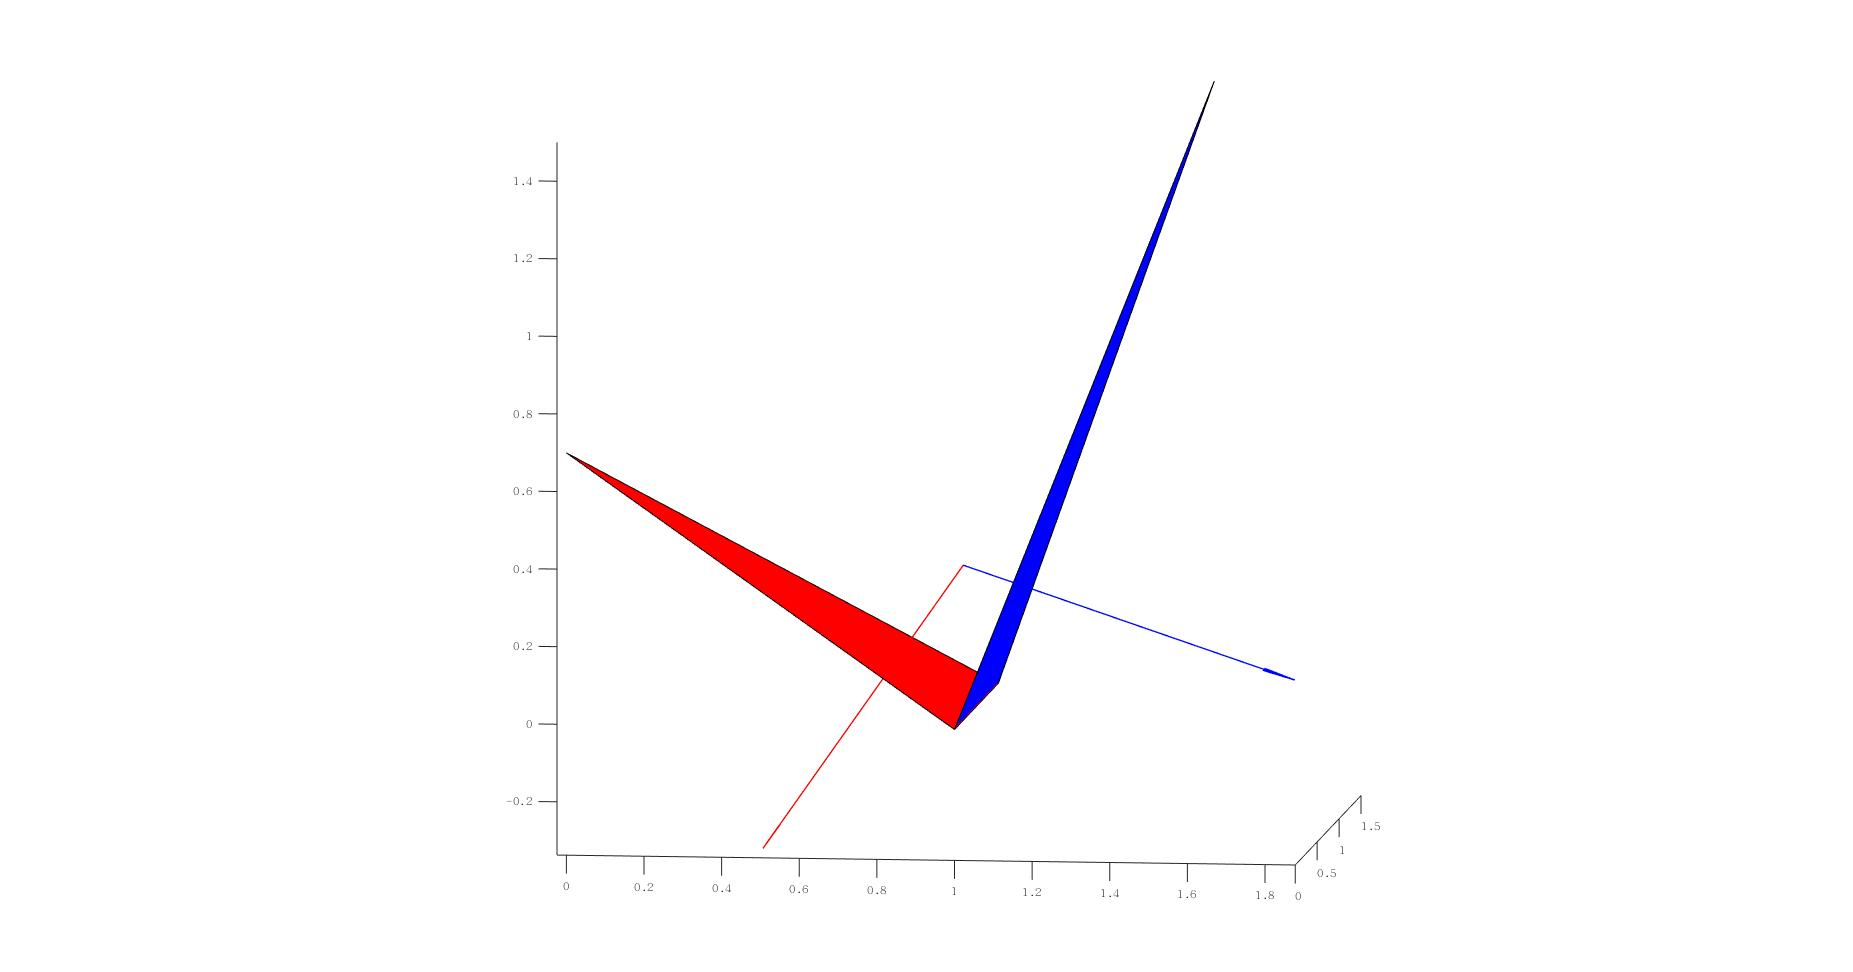
\includegraphics[width=10cm]{fig/nearsituation1.jpg}
	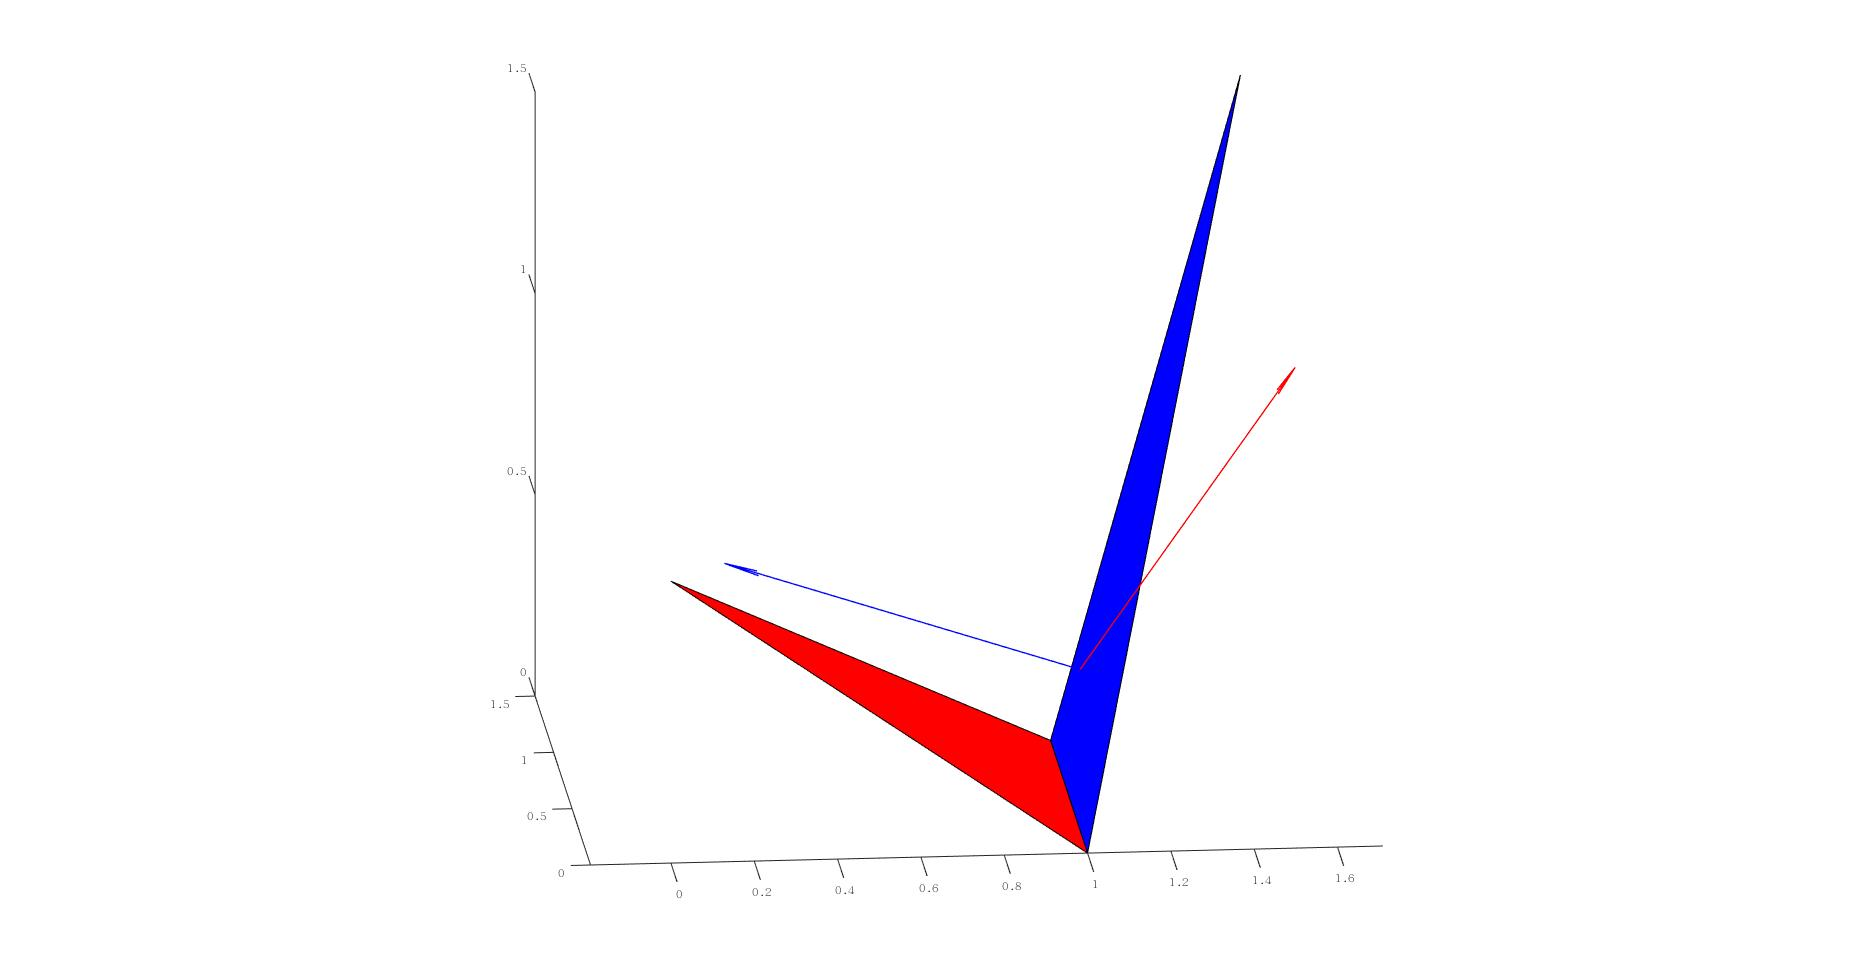
\includegraphics[width=10cm]{fig/nearsituation2.jpg}
\end{figure}

容易得到第一种情况平面之间的夹角$\beta = \pi - \alpha$,另一种情况$\beta = 3 \pi - \alpha$.
5-21行输出与三角形tri以seg为公共边的所有三角形计算所需旋转的角度$angle$并输出
最小$angle$的三角形,即相邻的三角形.

\subsection{算法10: 判断点与Yinset之间的位置关系}

已知Yinset的边界为有限个闭曲面的粘合.所以Yinset边界将全空间分为有限个连通区域.
其中部分为Yinset内部,部分为外部.即只需判断点p在Yinset边界上,或被某个连通区域G包含,
连通区域G在Yinset内部或者外部.

判断连通区域在Yinset内部或外部可以通过Yinset的边界包含的G的边界.计算过程中边界是空间
三角形的集合.

通过点p发出一条射线r,与表示Yinset的边界的所有三角形求交,选取与p点最接近的交点q(算法3-4行)
若点p,q重合显然p在Yinset边界上(算法5-8行).当p,q不重合时,由最接近性质,线段pq(除q点)与Yinset边界
无交点,又因为Yinset边界将全空间划分为有限个连通区域,线段pq(除q点)内部是连通的,所以pq属于
同一个连通区域,而p属于连通区域G,所以pq属于G,因此q在G的边界上.

当tri是G的边界时,通过tri(G的边界)的法向量与pq的位置可以得到连通区域G是Yinset的内部或外部.
(程序27行),即q与Yinset的位置关系.(仅有当pq与tri平行时无法判断,当包含q点的所有三角形与
pq平行同时也包含q,此时pq内部必有与这些三角形的的重合点,与q为最近交点矛盾)

10-11行,包含q点的三角形只有tri时,因为tri包含G中在pq上的某些点序列的极限点,
所以tri只能是G的边界.

在程序13-34行中处理pq交三角形数量大于1时.对每个包含点q的三角形ta,取三角形内的线段dq,
满足角度$\angle pqd_{ta}$最小,计算所有包含点q的三角形,得到使得$\angle pqd_{tri}$最小的
所有三角形集合tris($\angle pqd_{tri} < \pi$,或者tri的三条边不能构成面积非0的三角形).
计算tris中的三角形tri满足$\triangle pqd_{tri},tri$沿着$qd_{tri}$
之间夹角最小.下证tri为连通区域G的边界

取tri和pq内部上充分接近q点的两点a,b,使得$\angle bqa$充分接近$\angle pqd_{tri}$.若线段ab内部与Yinset边界无交点,折线pba连通且只与Yinset
边界交于a,p.pba属于G且包含极限逼近tri内部点a的点序列,(所有表示Yinset边界的三角形
只有tri包含点j)所以tri是G的边界.若ab内部与Yinset边界中的三角形tri1相交与点c,显然有
$\angle pqa > \angle pqc$.
因为a,b都充分接近点q,因此tri1与q充分接近即tri1包含q.因
此q必在tri与tri1的边上,若$d_{tri}$在tri的内部,不妨令a在线段$qd_{tri}$上,此时
$\angle pqd_{tri} = \angle aqb > \angle aqc \geq \angle pqd_{tri1}$,与$\angle pqd_{tri}$矛盾.
所以$d_{tri}$在tri的边上.令a充分接近线段$qd_{tri}$可得tri1必包含$qd_{tri}$中的一段,
取tri1在$qd_{tri}$上一点e,由定义有$\angle pqd_{tri} = \angle pqe \geq \angle pqd_{tri1}$
因$\angle pqd_{tri}$是选出的最小的$\angle pqd_{tri} \leq \angle qpd_{tr1}$,结合可得
$\angle_{tri1} = \angle_{tri}$,由对称性,不妨令$d_{tri1} = e$.
$\angle aqb$投影到垂直于$qd_{tri}$的平面上,由tri和tri1都包含了$qd_{tri}$的一部分有内部点
a,c必不与q的投影重合,而$\angle pq_{tri} < \pi$知p与q不重合.综上$\angle pqa,\angle pqc$
的投影到$\triangle pqd_{tri}, \triangle pqd_{tri1}$, tri,tri1的公共边的垂直平面上,角度分别等于
三角形沿着$qd_{tri}$的夹角,而投影不改变角度之间的大小关系,所以$\angle pqa > \angle pqc$
即为$\triangle pqd_{tri1}, tri1$沿着$qd_{tri1}$之间的夹角更小,与tri的取法矛盾.
综上所述,tri是G的边界.



\begin{algorithm}  
	\caption{Yinset 求交算法}  
	\label{alg:1}
	\begin{algorithmic}[1] %每行显示行号    
		\renewcommand{\algorithmicrequire}{\textbf{Input : }}
		\Require $Yinset\ yinsetA,yinsetB$.
		\renewcommand{\algorithmicrequire}{\textbf{Precondition : }}
		\Require $yinsetA,yinsetB$ 的边界曲面已经完成三角划分
		\renewcommand{\algorithmicensure}{\textbf{Output : }}
		\Ensure $Yinset\ yinsetC$
		\renewcommand{\algorithmicensure}{\textbf{Postcondition : }}
		\Ensure $yinsetC$ 是$yinsetA,yinsetB$的交集,且边界曲面完成三角划分.
		\Function {Meet}{$yinsetA, yinsetB$}  
		\State Let $TriangleA,TriangleB$ be vector of $Triangle$, 
		\State $FaceA,FaceB$ be vector of $SurfacePatch$.
		$closeFaceC$ be vector of $GluingCloseSurface$.
		\State $TriangleA,TriangleB,IntersectInfo \gets \textbf{Collapse}(yinsetA,yinsetB)$. 
		% \State $TriangleIntersect\ funcIntersect()$
		\State $\textbf{TriangleIntersect}(TriangleA,TriangleB,IntersectInfo)$.
		% \For{$Triangle\ tria \in TriangleA, trib \in TriangleB$}
		% 	\State $funcIntersect(tria,trib)$
		% \EndFor
		% \State $IntersectInfo \gets pair(funcIntersect.resultA,funcIntersect.resultB$
		% \State $Triangulate funcTriangulate()$
		\State Let $TriangulA,TriangulB$ store Triangulation  result.
		\State $EdgeInfo \gets \textbf{Triangulate}(IntersectInfo,TriangleA,TriangleB,TriangulA,TriangulB)$.
		\State $vecTriA,vecTriB  \gets $
		\Statex \quad \  $\textbf{RemoveOverlap}(IntersectInfo,TriangleA,TriangleB,$
		$TriangulA,TriangulB,EdgeInfo)$.
		% \For{$triA,triB \in IntersectInfo.first, second$}
		% 	\State $TriangleA.erase(triA), TriangleB.$
		% 	\State $TriangleA.insert(funcTriangulate(triA))$
		% \EndFor
		\State $FaceA \gets \textbf{PrePast}(vecTriA,EdgeInfo.A), 
		FaceB \gets \textbf{PrePast}(vecTriB,EdgeInfo.B)$.
		\State $\textbf{Locate}(FaceA,TriangleB),\textbf{Locate}(FaceB,TriangleA)$.
		\State $closeFaceC \gets \textbf{Past}(FaceA + FaceB)$.
		\State $yinsetC \gets Yinset(closeFaceC)$. 
		\State $yinsetC.buildHass()$.
		\State \Return $yinsetC$. 
		\EndFunction
		\State
		\Function{Collapse}{$A,B$}
		\State $TriangleA \gets 0, TriangleB \gets 0$ . 
		\For{$Face\ fa \in A.vecFace, fb \in B.vecFace$}
		\For{$Triangle\ tria \in fa, trib \in fb$}
		\State $TriangleA[end] \gets tria $.
		\State $IntersectInfo.resultA[tria] \gets tria's edges$.
		\State $TriangleB[end] \gets trib$.
		\State $IntersectInfo.resultB[trib] \gets trib's edges$.
		\EndFor
		\EndFor
		\State \Return{$TriangleA,TriangleB$}.
		\EndFunction
	\end{algorithmic}
\end{algorithm}

\begin{algorithm}
	\caption{三维三角形求交算法}
	\begin{algorithmic}[1]
		\renewcommand{\algorithmicrequire}{\textbf{Input : }}
		\Require $vector< Triangle >\ TriangleA,TriangleB$.
		\renewcommand{\algorithmicrequire}{\textbf{Precondition : }}
		\Require None
		\renewcommand{\algorithmicensure}{\textbf{Output : }}
		\Ensure $ vector<pair<vector<Segment>,
		vector<vector<Triangle>::iterator>>> resultA,resultB$ 
		\renewcommand{\algorithmicensure}{\textbf{Postcondition : }}
		\Ensure $resultA$对应于$TriangleA$中相同下标的$tria$,
		$it.first$是$tri$与$TriangleB$中所有$Triangle$的交线段的集合,
		当$Triangle$之间重合时,输出边与另一个$Triangle$的交.
		$it.second$是$TriangleB$中与$tria$有重合部分的$Triangle$的集合.
		\Function{TriangleIntersect}{$TriangleA,TriangleB$}
		\State Let $resultA,resultB$ be empty vector.
		\For{$tria \in TriangleA$}
		\For{$trib \in TriangleB$}
		\State $\textbf{SingleCalculate}(tria,trib,resultA,resultB)$.
		\EndFor
		\EndFor
		\State \Return $resultA,resultB$.
		\EndFunction
		\State
		\Function{SingleCalculate}{$tria,trib,resultA,resultB$}
		\State Let $interLine$ be empty vector of $Line$.
		\State Get the $Plane pla,plb$ of the $Triangle tria,trib$.
		\If{$pla,plb$ is parallel.}
		\State Insert the lines on which the $Triangle\ tria,trib$ edges lie into $interLine$.
		\State $resultA[tria].second[end] \gets trib$.
		\State $resultB[trib].second[end] \gets tria$.
		\Else
		\State Insert the line which is intersection of $Plane\ pla,plb$ into $interLine$.
		\EndIf
		\For{$Line\ l \in interLine$}
		\State $sega \gets \textbf{intersectCoplane}(tria,l)$.
		\State $segb \gets \textbf{intersectCoplane}(trib,l)$.
		\State Get  the coincidence $Segment\ seg$ of $Segment\ sega,segb$.
		\State Set $seg$'s $neighbour$ is $tria,trib$. 
		\If{$seg$ longer than 0.}
		\State $resultA[tria].first[end] \gets seg$.
		\State $resultB[trib].first[end] \gets seg$.
		\EndIf
		\EndFor
		\State \Return
		\EndFunction
	\end{algorithmic}
\end{algorithm}

\begin{algorithm}
	\caption{共面三角形与直线求交}
	\begin{algorithmic}[1]
		\renewcommand{\algorithmicrequire}{\textbf{Input : }}
		\Require $Triangle\ tri$,$Line\ l$.
		\renewcommand{\algorithmicrequire}{\textbf{Precondition : }}
		\Require $tri$与$l$共面.
		\renewcommand{\algorithmicensure}{\textbf{Output : }}
		\Ensure $Segment\ seg$.
		\renewcommand{\algorithmicensure}{\textbf{Postcondition : }}
		\Ensure $seg$是$tri,l$的交集.当交集为空时输出默认构造长度为0的$seg$.
		\Function{intersectCoplane}{$tri,l$}
		\State According to normal vector of $tri$, project $tri$ and $l$ to a appropriate plane
		(xy-,yz- or xz-plane).
		\State Calculate coincident part $Segment<2> proseg$ of projection of $tri$ and $l$.
		\State Get the primary image $Segment<3> seg$ of $proseg$ in 3D space.
		\State \Return $seg$.
		\EndFunction
	\end{algorithmic}
\end{algorithm}

\begin{algorithm}
	\label{alg:4}
	\caption{寻找恰当的粘合三角形}
	\begin{algorithmic}[1]
		\renewcommand{\algorithmicrequire}{\textbf{Input : }}
		\Require $Triangle\ tri$,$Segment\ edge$.
		\renewcommand{\algorithmicrequire}{\textbf{Precondition : }}
		\Require $edge$是$tri$的边,$edge.neighbor$指向所有以$edge$为边的$Triangle$,
		$Triangle$集合中不存在共面的两个$Triangle$.
		\renewcommand{\algorithmicensure}{\textbf{Output : }}
		\Ensure $Triangle\ neartri$.
		\renewcommand{\algorithmicensure}{\textbf{Postcondition : }}
		\Ensure 按$tri$法向量方向绕$edge$反方向旋转,$edge.neighbor$中最早与$tri$重合的$Triangle$.
		\Function{FindNearTriangle}{$edge,tri$}
		\State Assign norm vector of $tri$ to $Vec\ normtri$.
		\State Get Direction $Vec observe$ of $edge$ in $tri$.
		\State $bestangle \gets 2*PI$,$neartri \gets 0$.
		\For{$neightri \in edge.neighbor$}
		\If{$neightri$'s direct on $edge$ opposite to $tri$'s}
		\State Assign norm vector of $neightri$ to $normneightri$.
		\State $angle \gets atan2(cross(normtri,normneightri).norm(), dot(normtri,normneightri))$.
		\If{$dot(corss(normtri,normneightri),observe) < 0$}
		\State $angle \gets 2 * PI - angle$.
		\EndIf
		% \If{$bestangle < PI$}
		% \If{$(angle >= PI\  $?$  \ 1 $ : $ angle < bestangle$} 
		% \State $Break$.
		% \EndIf
		% \Else
		% \If{$angle >= PI\ \&\&\ angle < bestangle$}
		% \State $Break$.
		% \EndIf
		% \EndIf
		% \State $bestangle \gets angle, neartri \gets neightri$. 
		% \EndIf
		\If{$angle < PI$}
		\State $angle \gets PI - angle$.
		\Else
		\State $angle \gets 3 * PI - angle$.
		\EndIf
		\If{$angle < bestangle$}
		\State $bestangle \gets angle, neartri \gets neightri$. 
		\EndIf
		\EndIf
		\EndFor
		\State \Return $neightri$.
		\EndFunction
	\end{algorithmic}
\end{algorithm}


\begin{algorithm}
	\caption{三角划分算法}
	\begin{algorithmic}[1]
		\renewcommand{\algorithmicrequire}{\textbf{Input : }}
		\Require $IntersectInfor$, $vector<Triangle>$ $TriangleA,TriangleB$.
		\renewcommand{\algorithmicrequire}{\textbf{Precondition : }}
		\Require $IntersectInfor$中的$resultA.first$是$TriangleA$
		相同下标的$tria$与$TriangleB$中所有$Triangle$的交线段和共面$Triangle$的集合.
		$resultA.second$是与$tria$有重合部分的$trib \in TriangleB$
		$resultB$同样.
		\renewcommand{\algorithmicensure}{\textbf{Output : }}
		\Ensure $vector<vector<Triangle>> TriangulA,TriangulB$,
		$vector<vector<array<Segment>>>\ EdgeInfo.A,EdgeInfo.B$.
		\renewcommand{\algorithmicensure}{\textbf{Postcondition : }}
		\Ensure $TriangulA$存储$TriangleA$相同下标代表的$Triangle$的三角划分的$Triagnle$集合.
		保证重合部分的三角划分一致.
		% \Ensure $TriangleA,TriangleB$删除在$resultA,resultB$中交线段信息非空的$Triangle tri$,
		% 并分别插入$tri$三角化后的细分$Triangle$.同时处理重合$Triangle$对,若同向只
		% 删除$TriangleB$中的重合$Triangle$,若异向$TriangleA$中的重合$Triangle$也删除
		\Function{Triangulate}{$IntersectInfo,TriangleA,TriangleB$}
		% \State Let $swapA,swapB$ be empty vector of $Triangle$.
		\State $intersectInfoA,intersectInfoB \gets IntersectInfo.resultA,IntersectInfo.resultB$.
		\For{$tria \in TriangleA$}
		\If{$intersectInfoA.first,intersectInfoB.second$ is not empty.}
		\State $EdgeInfo.A[tria]$
		\Statex \qquad \qquad \quad $\gets $\textbf{SingleTriangulate}($tria,intersectInfoA[tria],TriangulA[tria],IntersectInfoB$).
		\EndIf
		\EndFor
		\For{$trib \in TriangleB$}
		\If{$intersectInfoB.first,intersectInfoB.second$ is not empty.}
		\State $EdgeInfo.B[trib] \gets $\textbf{SingleTriangulate}($trib,intersectInfoB[trib],TriangulB[trib]$).
		\EndIf
		\EndFor
		\State \Return $TriangulA,TriangulB,EdgeInfo$.
		\EndFunction
		\State
		\Function{SingleTriangulate}{$tria,IntersectInfoA[tria],TriangulA[tria],IntersectInforB$}
		\State Let $newEdge$ be vector of $Segment$ after Triangulation.
		\State Project all $Segment$ to a appropriate plane.
		\State $newEdge \gets \textbf{AddSegment}(IntersectInfoA[tria])$
		\If{$newEdge$ is not trival \textbf{And} $IntersectInfoA[tria]$'s Overlap $Triangle$ is not empty}
		\For{$trib \in IntersectInfoA[tria].second$}
		\For{$seg \in newEdge$}
		\If{$trib$ contain $seg$}
		\State Add $trib$ into $seg$'s neighbor.
		\State $IntersectInfoB.first[end] \gets seg$.  
		\EndIf
		\EndFor
		\EndFor
		\EndIf
		\State \Return \textbf{GeneratePolygon}($newEdge,TirangulA[tria]$).
		\EndFunction
	\end{algorithmic}
\end{algorithm}

\begin{algorithm}
	\caption{$\textbf{AddSegment}(segs)$}
	\begin{algorithmic}[1]
		\renewcommand{\algorithmicrequire}{\textbf{Input : }}
		\Require $segs$, vector of $Segment$ in 2D space.
		\renewcommand{\algorithmicrequire}{\textbf{Precondition : }}
		\Require None
		\renewcommand{\algorithmicensure}{\textbf{Output : }}
		\Ensure $newEdge$, vector of $Segment$.
		\renewcommand{\algorithmicensure}{\textbf{Postcondition : }}
		\Ensure $newEdge$ 将平面划分为一个无界区域和一些三角形.
		\Function{AddSegments}{$segs$}
		\State 三角划分算法.
		\EndFunction
	\end{algorithmic}
\end{algorithm}

\begin{algorithm}
	\caption{消除重合的三角面片}
	\begin{algorithmic}[1]
		\renewcommand{\algorithmicrequire}{\textbf{Input : }}
		\Require $IntersectInfo,$
		$vector<Triangle> TriangleA,TriangleB,$
		$vector<vector<Triangle>> TriangulA,TriangulB$.
		\renewcommand{\algorithmicrequire}{\textbf{Precondition : }}
		\Require $intersectInfo.resultA.second$包含$TriangleA$中相同下标
		的$tria$重合的所有$TriangleB$中的$Triangle$.$TriangulA$一一对应于$TriangleA$
		求交后的三角划分结果.重合曲面部分的三角划分完全一致,即重合部分的小三角形顶点位置一致
		\renewcommand{\algorithmicensure}{\textbf{Output : }}
		\Ensure $vector<Triangle> vecTriA,vecTriB$.
		\renewcommand{\algorithmicensure}{\textbf{Postcondition : }}
		\Ensure $vecTriA,vecTriB$包含三角划分后的结果.
		重合部分若法向量一致只保留$TriangleA$中的三角划分,若相反重合部分的三角划分都不保留.
		\Function{RemoveOverlap}{$IntersectInfo,TriangleA,TriangleB,TriangulA,TriangulB$}
		\State Let $OverlapA$ represent $IntersectInfo.resultA$.
		\For{$tria \in TriangleA$}
		\If($Overlap.second$ is not empty)
		\For{$trib \in Overlap.second$}
		\For{$smalltria \in TriangulA$}
		\State Find $smalltrib$ in $TriangulB$ success $smalltrib == smalltria$.
		\If{$tria,trib$ have contrary normal direc}
		\State $TriangulA[tria].erase(smalltria)$.
		\State $IntersectInfo.resultA[tr]$
		\EndIf
		\State $TriangulB[trib].erase(smalltrib)$.
		\EndFor
		\EndFor
		\EndIf
		\EndFor
		\State  Insert all $Triangle$ in $TriangulA,TriangulB$ to $vecTriA,vecTrib$ respectively.
		\State Correct $EdgeInfo$'s order respect $vecTriA,vecTriB$.
		\State \Return $vecTriA,vecTriB$.
		\EndFunction
	\end{algorithmic}
\end{algorithm}


\begin{algorithm}
	\caption{预粘合算法}
	\begin{algorithmic}[1]
		\renewcommand{\algorithmicrequire}{\textbf{Input : }}
		\Require $vector<Triangle>\ TriangleA, vector<array<Segment>> EdgeInfo$.
		\renewcommand{\algorithmicrequire}{\textbf{Precondition : }}
		\Require $\forall tria \in TriangleA$,$tria$的边$EdgeInfo[tria]$中的$seg.neighbor$存储有所有以$seg$
		为边的$Triangle$. 并且$tria.yin$记录求交算法前属于的$yinset$.
		\renewcommand{\algorithmicensure}{\textbf{Output : }}
		\Ensure $FaceA$是$GluingCloseSurface$和$SurfacePatch$的集合.
		\renewcommand{\algorithmicensure}{\textbf{Postcondition : }}
		\Ensure $FaceA$中的$GluingCloseSurface$等于
		$yinsetA$的$vecFace$中与$yinsetB$中的面无交集的子集集合.
		另一部分$SurfacePatch$是由另一部分$yinsetA.vecFace$子集沿与$yinsetB$表面的交
		进行切割后的曲面片,即曲面片的边界$boundary$是$yinsetA,yinsetB$的表面的交线.
		(曲面重合情况在\textbf{RemoveOverlap}中移除).
		\Function{PrePast}{$TriangleA$}
		\State Let $FaceA.gCSface$ be empty vector of $GluingCloseSurface$,
		$FaceB.SfacePatch$ be empty vector of $SurfacePatch$.
		\State Empty set $F,T$ of $Triangle$.Insert every $Triangle$ in $TriangleA$ into $T$,
		\State Empty set $vecF$ of $Triangle$,Empty vector $boundary$ of $Segment$. 
		\State $F.insert(T.begin()), T.erase(T.begin())$.
		\While{$T$ is not empty}
		\State $tria \gets F.begin(),F.erase(tria)$.
		\State $vecF.insert(tria)$.
		\For{$e \in EdgeInfo[tria]$}
		\State $neartri \gets \textbf{FindNearTriangle}(e,tria)$.
		\If{$neartri.inFace$ equal $tria.inFace$}
		\If{$vecF$ is not contain $neartri$}
		\State $F.insert(neartri)$.
		% \State $vecF.insert(neartri)$.
		\State $T.erase(neartri)$.
		\EndIf
		\Else
		\State $boundary.insert(pair(e,tria))$.
		\EndIf
		\EndFor
		\If{$F$ is empty}
		\If{$boundary$ is empty}
		\State $FaceA.gCSface[end] \gets GluingCloseSurface(vecF)$.
		\Else 
		\State $FaceA.SfacePatch[end] \ gets SurfacePatch(vecF,boundary)$.
		\State Empty $boundary$.
		\EndIf
		\State Empty $vecF$.
		\If{$T$ is empty}
		\State $Break$.
		\EndIf
		\State $F.insert(T.begin()), T.erase(T.begin())$.
		\EndIf
		\EndWhile
		\EndFunction
	\end{algorithmic}
\end{algorithm}

\begin{algorithm}
	\caption{选取求交后Yinset表面上的曲面}
	\begin{algorithmic}[1]
		\renewcommand{\algorithmicrequire}{\textbf{Input : }}
		\Require $GluingCloseSurface$ or $SurfacePatch$ $FaceA$,$vector<Triangle>\ TriangleB$.
		\renewcommand{\algorithmicrequire}{\textbf{Precondition : }}
		\Require $TriangleB$包含$Yinset yinsetB$的表面上的所有$TriangleB$.
		\renewcommand{\algorithmicensure}{\textbf{Output : }}
		\Ensure $FaceA$
		\renewcommand{\algorithmicensure}{\textbf{Postcondition : }}
		\Ensure 保留$FaceA$中在$Yinset\ yinsetB$内的曲面片.
		\Function{Locate}{$FaceA,TriangleB$}
		\State Name $vector<Point>\ vpa$, $array<char>\ vb$.
		\For{$fa \in FaceA$}
		\State Select $Triangle\ tria \in fa$.
		\State Get  center of gravity $pa$ of $tria$.
		\State $vpa[end] \gets pa$.
		\EndFor
		\State $vb \gets \textbf{LocatePoint}(vp,TriangleB)$
		\For{$b \in vb$}
		\If{$b$ is '$o$'}
		\State $FaceA.erase(fa)$.
		\EndIf
		\EndFor
		\EndFunction
	\end{algorithmic}
\end{algorithm}


\begin{algorithm}
	\caption{判断点与Yinset之间的位置关系}
	\begin{algorithmic}[1]
		\renewcommand{\algorithmicrequire}{\textbf{Input : }}
		\Require $vector<Point> vpa $,$vector<Triangle>\ TriangleB$.
		\renewcommand{\algorithmicrequire}{\textbf{Precondition : }}
		\Require $TriangleB$包含$Yinset yinsetB$的表面上的所有$TriangleB$.
		\renewcommand{\algorithmicensure}{\textbf{Output : }}
		\Ensure $string\ vb$
		\renewcommand{\algorithmicensure}{\textbf{Postcondition : }}
		\Ensure 当$vb$使用'i','o','b'分别标记$vpa$中的点在$yinsetB$的内部,外部和边界上.
		\Function{DetachalongBoundary}{$vecF$}
		\For{$p \in vpa$}
		\State Get arbitrary $Line l$ cross $p$.
		\State Intersect $l$ with every $Triangle$ in $TriangleB$, 
		Select the closest intersection $q$.
		\If{$q == p$}
		\State $vb[p] \gets 'b'$.
		\State $Break$.
		\EndIf
		\State $vqp \gets (p - q)/ \lVert p - q \rVert,normtri \gets 0$.
		\If{$vecTri$ contains only one $Triangle \ tri$}
		\State $normtri \gets$ normal vector of $tri$.
		\Else
		\State $smallangle = 1$
		\For{$tri$ In $vecTri$}
		\State Project segment $pq$ into the Plane that contains $tri$ get $pjpq$.
		\If{$pjpq \cap tri - q$ is not empty}
		\State Let $Point \ d$ be arbitrary point in $pjpa - q$.
		\State $angle \gets \angle pqd$.
		\Else
		\State Let $Point\ a,b,c$ be vertex of $tri$ except coincident with $q$.
		\State $(angle,d) \gets \min((\angle pqa,a), (\angle pqb,b), (\angle pqc,c))$.
		\EndIf
		\If{$angle == smallangle$}
		% \State Assuming $tri$'s edge  $Segment seg$ contain $q,d$.	
		\State Triangle vector $tris$ add $tri$ and $segs$ add $qd$.
		\EndIf
		\State $(smallangle,tris) \gets angle < smallangle $ ? $ (angle,tri), $ : $ (smallangle,tris)$.
		\EndFor
		\If{$tris$ contains only one Triangle $tri$}
		\State  $normtri \gets$ normal vector of $tri$.
		\Else
		\State Get $tri$ in $tris$ such that angle between $tri$ and $pqd$ is smallest.
		\State $normtri \gets$ normal vector of $tri$.
		\EndIf
		\EndIf
		\State $vb[p] \gets dot(vqp,normtri) $ ? $ 'o' $ : $ 'i' $.
		\EndFor
		\State \Return $vb$.
		\EndFunction
	\end{algorithmic}
\end{algorithm}


\begin{algorithm}
	\caption{曲面片之间的粘合算法}
	\begin{algorithmic}[1]
		\renewcommand{\algorithmicrequire}{\textbf{Input : }}
		\Require $GluingCloseSurface$和$SurfacePatch$的集合$vecF$.
		\renewcommand{\algorithmicrequire}{\textbf{Precondition : }}
		\Require $vecF$中的曲面片,交且仅交于$boundary$上.
		\renewcommand{\algorithmicensure}{\textbf{Output : }}
		\Ensure $GluingCloseSurface\ closeFaceC$.
		\renewcommand{\algorithmicensure}{\textbf{Postcondition : }}
		\Ensure $closeFaceC$中的所有面都是有向曲面,自相交区域不包含闭合曲线,
		且两两之间的交集是1维CW复形.
		\Function{Past}{$vecF$}
		% \State $\textbf{DetachNonCycleBoundary}(vecF)$.
		\State Set $set<int> connectFace,allF, vector<int> pastFace$.
		\State Empty $set<Segment> pastBoundary$.
		\State Insert all index of $Face$ in $vecF$ into $allF$. 
		\State $connectFace.insert(allF.begin()), allF.erase(allF.begin())$.
		\While{$allF$ is not empty \textbf{Or} $connnectF$ is not empty}
		\State $f \gets vecF[connectF.begin()], connectF.erase(f)$.
		\State $pastFace.insert(f)$.
		\For{$seg \in f.neighbor$}
		\State Get $Triangle\ tri$ in $f$ and contain $seg$.
		\State $neartri \gets \textbf{FindNearTriangle}(seg,tri)$.
		\If{$neartri.inFace$ not in $pastFace$}
		\State $connectFace.insert(neartri.inFace)$.
		\State $allF.erase(neartri.inFace)$
		\EndIf
		\EndFor
		\If{$connectF$ is empty}
		\State $closeFaceC[end] \gets SurfacePatch(vecF[pastFace])$.
		\State Empty $pastFace$
		\If{$allF$ is empty}
		\State $Break$.
		\EndIf
		\State  $connectFace.insert(allF.begin()), allF.erase(allF.begin())$.
		\EndIf
		\EndWhile
		% \State $\textbf{DetachalongBoundary}(closeFaceC)$.
		\State \Return $closeFaceC$.
		\EndFunction
	\end{algorithmic}
\end{algorithm}

% \begin{algorithm}
	% 	\caption{将自相交曲面沿非流形点剪开算法}
	% \begin{algorithmic}[1]
		% 		\renewcommand{\algorithmicrequire}{\textbf{Input : }}
		% 		\Require $GluingCloseSurface$和$SurfacePatch$的集合$vecF$.
		% 		\renewcommand{\algorithmicrequire}{\textbf{Precondition : }}
		% 		\Require $vecF$中的曲面片互相之间不相交,
		% 		可能自交但仅自交交于$boundary$上,且每个曲面都是可定向的.
		% 		\renewcommand{\algorithmicensure}{\textbf{Output : }}
		% 		\Ensure $GluingCloseSurface\ closeFaceC$.
		% 		\renewcommand{\algorithmicensure}{\textbf{Postcondition : }}
		% 		\Ensure $closeFaceC$中的所有面都是可定向曲面,且不自相交.即将$vecF$中的曲面片
		% 		沿着1维CW复形$boundary$剪开.
		% 		\Function{DetachalongBoundary}{$vecF$}
		% 		\State 自相交曲面不知道该怎么剪开.
		% 		\EndFunction
		% 	\end{algorithmic}
		% \end{algorithm}
		
		
		
		
		\end{document}
		
		
		%%% Local Variables: 
		%%% mode: latex
		%%% TeX-master: t
		%%% End: 
		
		% LocalWords:  FPN underflows denormalized FPNs matlab eps IEEE iff
		% LocalWords:  cardinality significand quadratically bijection unary
		%  LocalWords:  contractive bijective postcondition invertible arity
		%  LocalWords:  subspaces surjective injective monomials additivity
		%  LocalWords:  nullary Abelian abelian finitary eigenvectors adjoint
		%  LocalWords:  eigenvector nullspace Hermitian unitarily multiset
		%  LocalWords:  nonsingular nonconstant homomorphism homomorphisms
		%  LocalWords:  isomorphically indeterminates subfield isomorphism
		%  LocalWords:  nondefective diagonalizable contrapositive cofactor
		%  LocalWords:  submatrix nilpotent positivity orthonormal extremum
		%  LocalWords:  Jacobian nonsquare semidefinite nonnegative RHS LLS
		%  LocalWords:  roundoff closedness
		